\section{Business understanding} \label{seq:business}

 In this step the objective is to determine and understand the context and the scope of the project. So it has a lot in common with the initial steps of any significant project undertaking.

 \subsection{Determine Business Objectives}


\begin{figure}[h]
    \includegraphics[width=\linewidth]{res/RL}
    \caption{One of the main Rocket League artworks}
\end{figure}

In recent years video games gained a lot of popularity, above all, multiplayer games; some of this are considered competitive and many sportive events take place around them.
Rocket League is a multiplayer competitive online game which is an hybrid that unifies soccer with car race games.

Thus, each match follows more or less soccer rules, but instead of human players there are cars controlled by the players. The number of players per team can be 1 (duel), 2, or 3 (standard). In our study we will focus on the main modality, that is 3vs3.

\subsubsection{Ranking System}

\begin{figure}[h]
    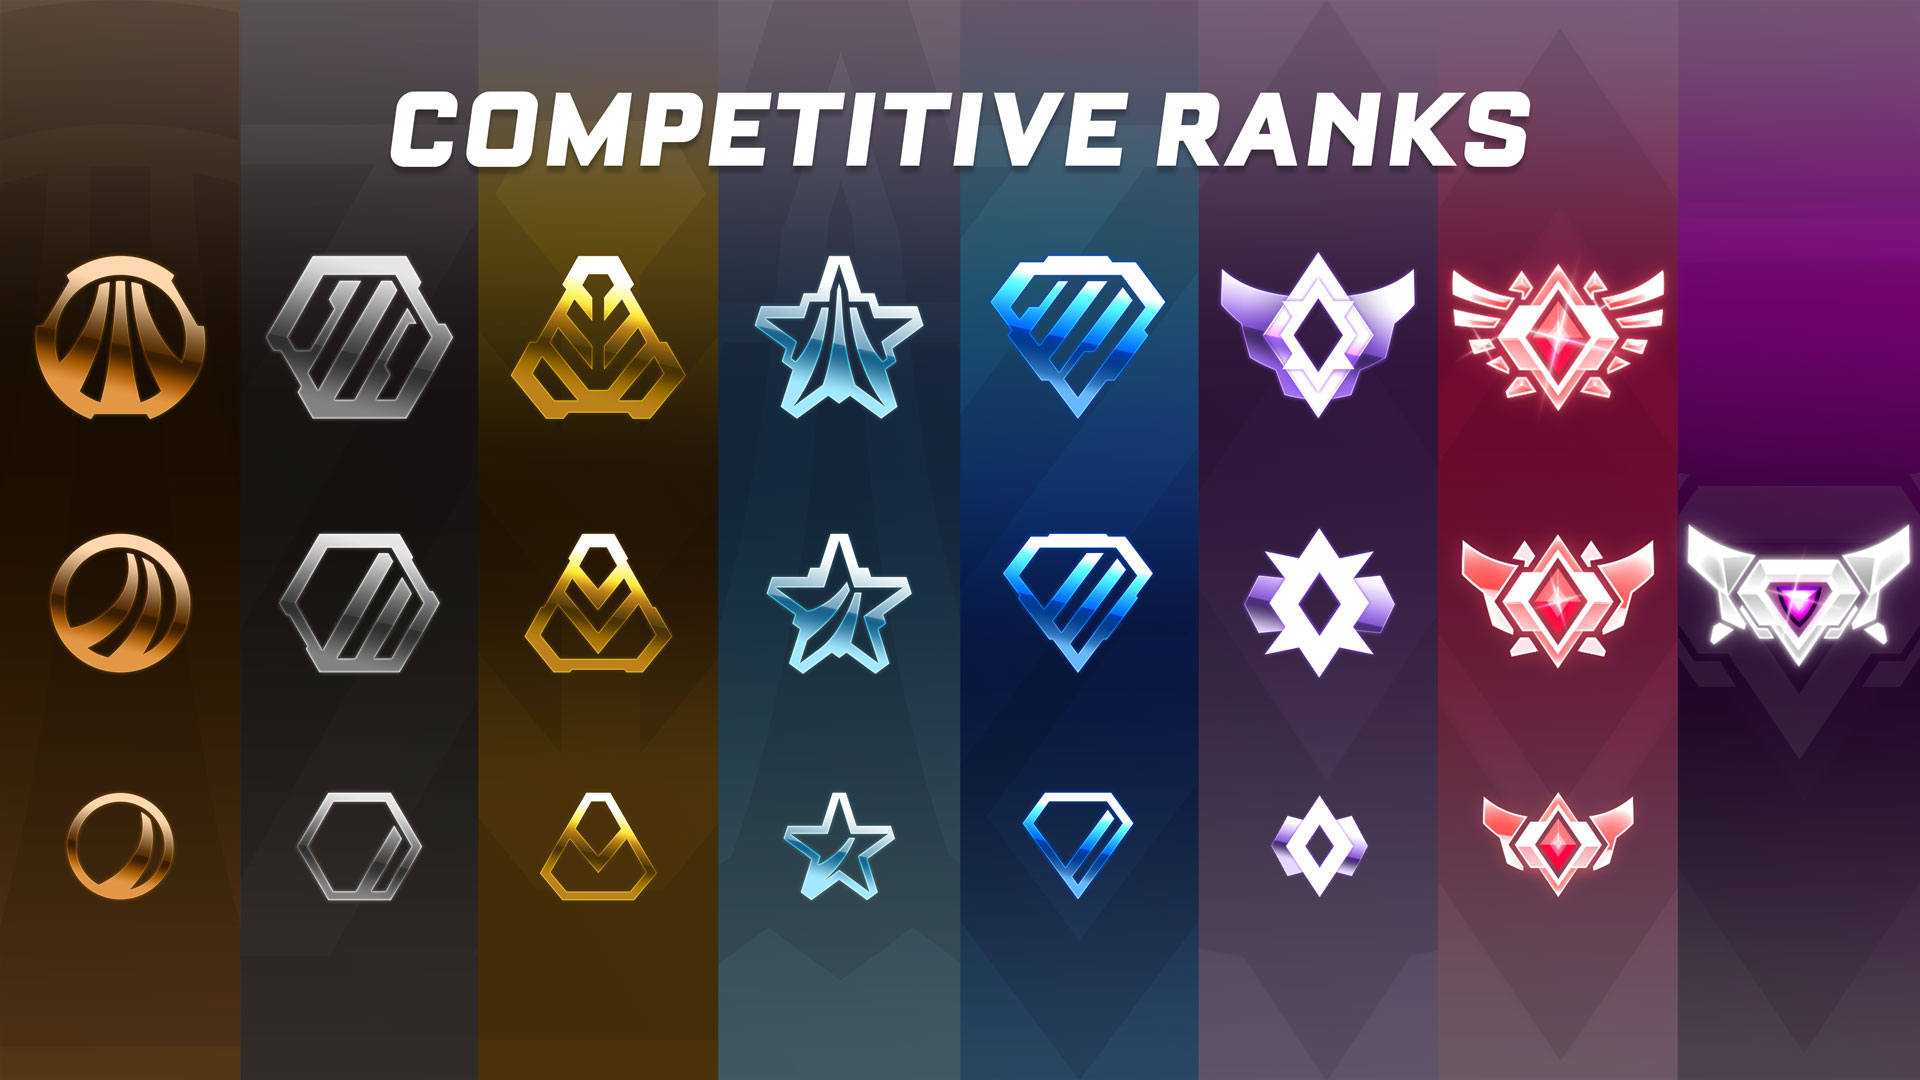
\includegraphics[width=\linewidth]{res/rankings}
    \caption{Rocket league rankings}
    \label{fig:ranks}
\end{figure}

In each modality, the player, after playing 10 online matches, is classified into a rank, based on the result of the 10 played matches. The ranks (visually shown in \reffig{fig:ranks}) are: 


\begin{multicols}{3}
    \begin{itemize}
        \item Bronze I
        \item Silver I
        \item Gold I
        \item Platinum I      
        \item Diamond I        
        \item Champion I         
        \item Grand Champion I    
        \item Bronze II
        \item Silver II
        \item Gold II       
        \item Platinum II     
        \item Diamond  II         
        \item Champion II         
        \item Grand Champion II
        \item Bronze III
        \item Silver III
        \item Gold III    
        \item Platinum III     
        \item Diamond  III        
        \item Champion III         
        \item Grand Champion III
    \end{itemize}
\end{multicols}

\begin{itemize}
    \item Supersonic Legend
\end{itemize}

Each rank, is split in four divisions (Division I, II, III and IV). And, each rank with its divisions is itself a discretization of a number, that is the Match Making Ranking (MMR). 
The MMR goes from 0 to potentially infinity, however the last rank: Supersonic Legend, takes the interval [1861, +Infinity]. A detailed view on MMRs and rankings is shown in \reftab{tab:mmrs}.

When the player starts playing, it is assigned an MMR of 600, that correspond to Gold III Division II. The MMR increase or decrease basing on the outcome of the matches it plays, obviously if he wins it will increase, viceversa if he loses. How much it can gain or lose at the end of the match is based on the number of played matches. In the first match, the gain/loss is +/-150. In the second match the values is halved, in it logarithmically decrease, until after some dozen of matches, it converge to +/- 10.

With this system, the player, will be classified in its most appropriate rank after some matches and, therefore will compete with players of the same skill level.

Our business objectives are, therefore two:
\begin{itemize}
    \item Analyze the statistics of each player of a match and predict its rank based on the performances that he shown;
    \item Divide players into categories based on the statistics of the match
\end{itemize}
\begin{table}[]
    \begin{tabular}{|l|c|c|c|c|}
    \hline
    \textbf{Tier}                 & \multicolumn{1}{l|}{\textbf{Division I}} & \multicolumn{1}{l|}{\textbf{Division II}} & \multicolumn{1}{l|}{\textbf{Division III}} & \multicolumn{1}{l|}{\textbf{Division IV}} \\ \hline
    \textbf{Supersonic   Legend}  & 1.861 — 2.008                            & —                                         & —                                          & —                                         \\ \hline
    \textbf{Grand Champion   III} & 1.709 — 1.739                            & 1.745 — 1.773                             & 1.788 — 1.814                              & 1.832 — 1.860                             \\ \hline
    \textbf{Grand Champion   II}  & 1.575 — 1.598                            & 1.600 — 1.636                             & 1.638 — 1.660                              & 1.677 — 1.701                             \\ \hline
    \textbf{Grand Champion I}     & 1.435 — 1.458                            & 1.460 — 1.494                             & 1.498 — 1.527                              & 1.537 — 1.559                             \\ \hline
    \textbf{Champion III}         & 1.315 — 1.333                            & 1.335 — 1.366                             & 1.368 — 1.394                              & 1.402 — 1.420                             \\ \hline
    \textbf{Champion II}          & 1.195 — 1.213                            & 1.215 — 1.246                             & 1.248 — 1.275                              & 1.282 — 1.300                             \\ \hline
    \textbf{Champion I}           & 1.075 — 1.093                            & 1.095 — 1.127                             & 1.128 — 1.148                              & 1.162 — 1.180                             \\ \hline
    \textbf{Diamond III}          & 995 — 1.003                              & 1.004 — 1.027                             & 1.028 — 1.051                              & 1.052 — 1.060                             \\ \hline
    \textbf{Diamond II}           & 915 — 923                                & 924 — 947                                 & 948 — 971                                  & 972 — 980                                 \\ \hline
    \textbf{Diamond I}            & 835 — 843                                & 844 — 867                                 & 868 — 891                                  & 892 — 900                                 \\ \hline
    \textbf{Platinum III}         & 773 — 778                                & 779 — 797                                 & 798 — 816                                  & 817 — 825                                 \\ \hline
    \textbf{Platinum II}          & 715 — 718                                & 719 — 737                                 & 738 — 756                                  & 757 — 765                                 \\ \hline
    \textbf{Platinum I}           & 655 — 658                                & 659 — 677                                 & 678 — 696                                  & 697 — 705                                 \\ \hline
    \textbf{Gold III}             & 595 — 598                                & 599 — 617                                 & 618 — 636                                  & 637 — 643                                 \\ \hline
    \textbf{Gold II}              & 535 — 538                                & 539 — 557                                 & 558 — 576                                  & 577 — 585                                 \\ \hline
    \textbf{Gold I}               & 475 — 478                                & 479 — 497                                 & 498 — 516                                  & 517 — 524                                 \\ \hline
    \textbf{Silver III}           & 415 — 418                                & 419 — 437                                 & 438 — 456                                  & 457 — 467                                 \\ \hline
    \textbf{Silver II}            & 355 — 358                                & 359 — 377                                 & 378 — 396                                  & 397 — 414                                 \\ \hline
    \textbf{Silver I}             & 295 — 298                                & 299 — 317                                 & 318 — 336                                  & 337 — 354                                 \\ \hline
    \textbf{Bronze III}           & 235 — 238                                & 239 — 257                                 & 258 — 276                                  & 277 — 290                                 \\ \hline
    \textbf{Bronze II}            & 172 — 178                                & 179 — 197                                 & 198 — 216                                  & 217 — 233                                 \\ \hline
    \textbf{Bronze I}             & 0 — 118                                  & 121 — 137                                 & 140 — 155                                  & 157 — 172                                 \\ \hline
    \end{tabular}
    \caption{MMRs intervals related to each Division and Rank in Rocket League}
    \label{tab:mmrs}
\end{table}

This work will result in a system able to measure the skill shown in a match for each player, and in a categorization useful to analyze the play styles.

\subsection{Determine Data Mining Goals}
\label{sec:min_goal}
The first goal is a classification/regression task. It is important to establish the granularity of the output. It is impossible to carefully determine each Division as they can change from a match to another, therefore the minimum granularity is the rank; however we still have 22 classes, that is quite high for a classification task. Thus, we could increase granularity by considering only the ranks without levels e.g. Silver instead of Silver II. We can see also this task as regression, as we can predict the MMR. We could also predict the MMR and then discretize into ranks.

The criteria will be based on accuracy and F1 score, we will accept an accuracy higher than 0.7.

The second goal is a clustering task. In this case the success criteria is qualitative, the objective is to define a categorization of play styles, therefore if the recognized clusters and centroids have a significant meaning we can consider the task fulfilled.